% 1. Introduction: Why is low power clock network important. Papers on how much energy is consumed by clock and how much can be saved
% 2. "old"-not-low power clock tree synthesis
% (3. 2D routing algorithm)
% 3. Possibilities to reduce clock power.
% 3.1 Use unbuffered trees
% 4. Clock networks for 3D stacked ICs. Different algorithms
% 4.1 Present algorithm from X. Zhang.
% 5. Conclusion

\documentclass[conference]{IEEEtran}
\IEEEoverridecommandlockouts
% The preceding line is only needed to identify funding in the first footnote. If that is unneeded, please comment it out.
\usepackage{cite}
\usepackage{amsmath,amssymb,amsfonts}
\usepackage{algorithmic}
\usepackage{graphicx}
\usepackage{textcomp}
\RequirePackage[utf8]{inputenc}
\def\BibTeX{{\rm B\kern-.05em{\sc i\kern-.025em b}\kern-.08em
    T\kern-.1667em\lower.7ex\hbox{E}\kern-.125emX}}
\begin{document}

\title{Low power reduction techniques for Ultra Low Power ProcessorsIoT applications}

\author{
	\IEEEauthorblockN{Karthik Sukumar}
	\IEEEauthorblockA{\textit{Department of Electrical and Computer Engineering}\\
	\textit{Technical University Munich (TUM)}\\Munich,
    Germany\\karthik.sukumar@tum.de}
}

\maketitle

\begin{abstract}
In this report the work of J.Zhou et al. \cite{b1} and J.Tang et al. \cite{b2}
on design techniques for an ultra low-power processor.

J.Zhou et al. focusses on Near-Threshold processor design for Ultra low power
processors. The paper discusses the challenges, performance issue and solutions
of the above.

J.Tang et al. discusses a case study by using GPS to demonstate that an
Ultra-low power processor used along with a heavy applications processor can
lead to further power savings.
\end{abstract}

\begin{IEEEkeywords}
Near threshold, Ultra low power, GPS, Offload Co-processor, Interrupt service
routines
\end{IEEEkeywords}

\section{Introduction} \label{sec:introduction}
Clock tree networks consume a large part of the overall power needed by an IC. The named values vary from 25\% \cite{b4} to 50\% \cite{b5}. There are several possibilities to reduce the power consumed by the clock network.

One of the most popular methods is voltage scaling due to its quadratic savings ($P_{dyn}=fC_LV_{DD}^2$). The used voltage in ultra-low voltage (ULV) applications is close to the threshold voltage ($V_T$). This saves energy, but makes the design less robust and susceptible to MOSFET process variations \cite{b6}.
The way to achieve a low-voltage clock tree with a minimzed and well-defined skew and with a well-controlled slew is discussed in \cite{b1}. The findings of \cite{b1} are presented in section \ref{sec:ulv_design}.  

Another approach to reduce the power consumed by the clock network is to optimize the network topolgy. While the skew control was well studied in two dimesional ICs \cite{b7}, the optimal topology in nowadays 3D stacked ICs is still being investigated. Through-silicon vias (TSVs) are used for the connection of clock networks on different dies. The impact of the TSV resistance-capacitance (RC) and the TSV count on the clock power, clock skew and clock skew is subject of \cite{b2}. The results of \cite{b2} are presented in section \ref{sec:tsv_design}.

\section{Ultra-Low Voltage Clock Network Design} \label{sec:ulv_design}

Generally, there are multiple ways to design a clock network. These ways are shown in Fig. \ref{fig:network_topologies}. Connecting all sinks (a sink can be anything that needs a clock signal, e.g. flip-flops) without attempting to balance the different paths is called "signal-route". In contrast to that, the H-trees try to take this into account. It is obvious that the path length from the clock source to each sink becomes more equal the higher the H-tree's level is.

\begin{figure}[htbp]
	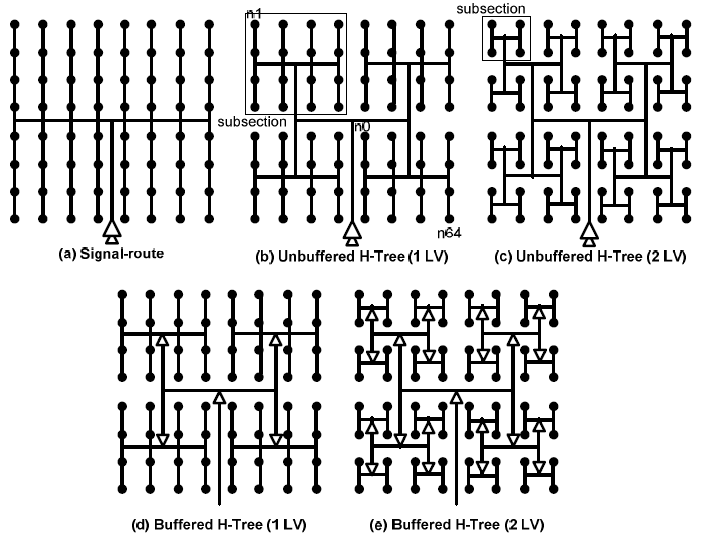
\includegraphics[width=\linewidth]{img/network_topologies.png}
	\centering
	\caption{Network topologies. Source: \cite{b1}}
	\label{fig:network_topologies}
\end{figure}

Furthermore, there is a difference between unbuffered and buffered H-trees. In unbuffered H-trees, the whole circuit is driven by a single driver, whereas in a buffered H-tree several smaller buffers are inserted to drive the tree. Normally, designers tend to use the buffered version, because then each driver has to drive a smaller RC-value and therefore the interconnect delay is mitigated, but as we will see later on this is not longer true for ULV applications.

\subsection{Clock networks behaviour without considering MOSFET process variations}
Energy consumption and clock skew can be simulated using SPICE. The simulation results for a 0.18$\mu m$ CMOS framework with 0.3$V$ supply voltage are shown in Fig. \ref{fig:skew_energy_normal}.\\
The skew decreases with the levels in tree as the paths to the sinks become more equal. This holds for both, the bufferd and unbuffered trees. The energy increases with the levels due to the overall wire length becoming larger. For higher tree levels, the bufferd version consumes less energy because the smaller buffers are more energy efficient in driving longer wires.

\begin{figure}[htbp]
	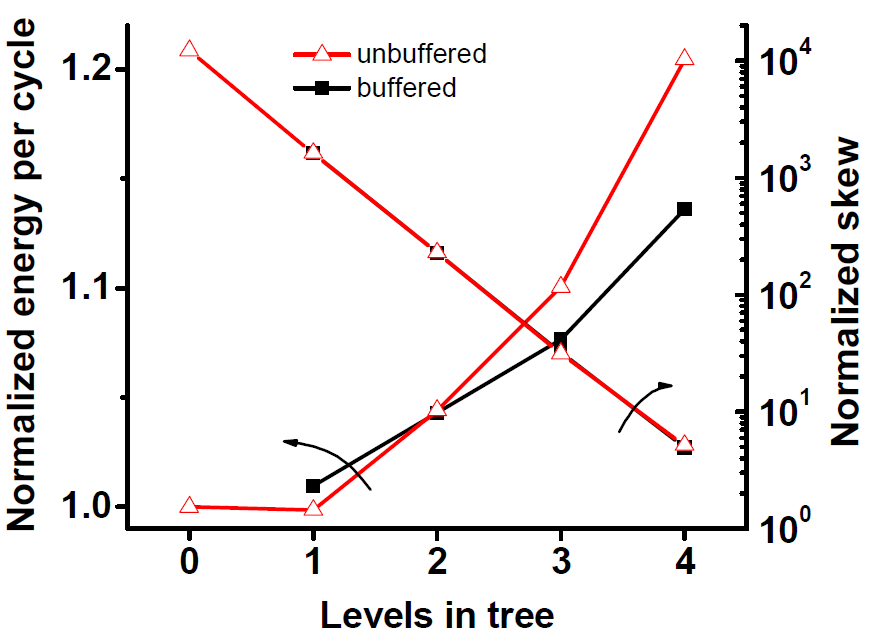
\includegraphics[width=0.8\linewidth]{img/skew_energy_normal.png}
	\centering
	\caption{Energy and skew over levels in tree. Simulated usinge SPICE without considering MOSFET process variations. Source: \cite{b1}}
	\label{fig:skew_energy_normal}
\end{figure}

\subsection{Clock networks behaviour with considering MOSFET process variations}
Since MOSFET process variations (e.g. random $V_{th}$ mismatch) have an exponential effect on gate delay at ULV circuits \cite{b8} this has to be considered. For this reason M. Seok et al. \cite{b1} performed Monte Carlo simulations with random MOSFET mismatch. The results are shown in Fig. \ref{fig:skew_slew_variations}. In contrast to the simulations without variations, the buffered trees perform much worse (Fig. \ref{fig:skew_slew_variations} (a)) in skew because the buffer delay is not anymore cancelled among buffers and starts to contribute to skew. The skew variability ($\sigma /\mu$) first decreases as more buffer stages are used with increasing tree level and thus the variations are averaged. But after level three it starts to increase again as smaller buffers are more sensitive to process variations.\\
The slew behaves similarly. The unbuffered version shows a good robustness while the buffered version behaves worse. The slew variability increases with the levels in tree. There is no averaging effect for the slew variability because the slew is mainly determined by the last buffer stage before the sink.

\begin{figure}[htbp]
	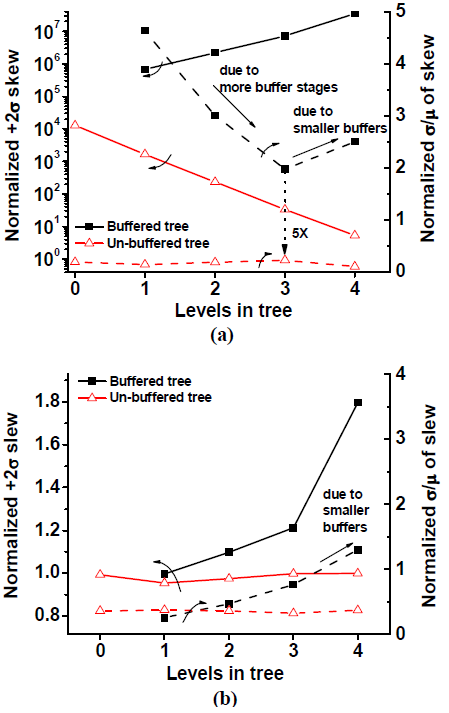
\includegraphics[width=0.8\linewidth]{img/skew_slew_variations.png}
	\centering
	\caption{Skew and slew over levels in tree with considering MOSFET process variations. Source: \cite{b1}}
	\label{fig:skew_slew_variations}
\end{figure}

\subsection{Adding buffers in ULV regimes}
In higher voltage regimes adding buffers to long interconnects often improves the interconnection delay (see Fig. \ref{fig:repeater}). For ULV applications this is not longer true, because the delay penalty for adding buffers is larger than the reduction of wire RC. As shown in Fig. \ref{fig:repeater} the version without repeater still performs better for a 30mm wire.

\begin{figure}[htbp]
	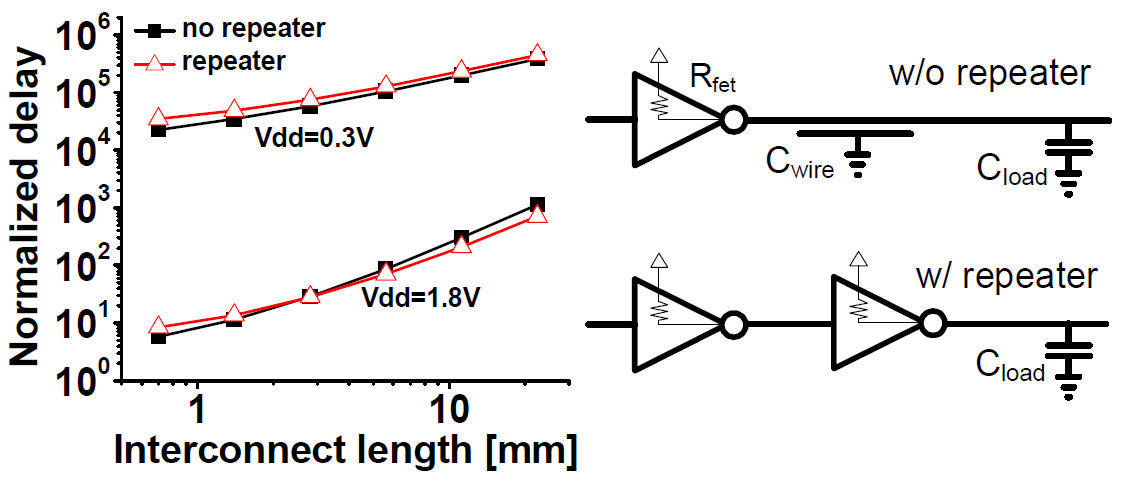
\includegraphics[width=0.8\linewidth]{img/repeater.png}
	\centering
	\caption{Driving long interconnects with and without repeaters at 0.3$V$ and 1.8$V$. Source: \cite{b1}}
	\label{fig:repeater}
\end{figure}


\section{Clock Network Design for Through-Silicon Via (TSV) Based 3D ICs} \label{sec:tsv_design}
Today's ICs are often built as 3D stacked ICs. The different dies are connected using through-silicon vias (TSVs). The 3D clock tree synthesis problem can therby be formulated as follows: Given are a set of sinks, a TSV bound (the user defined maximum of TSVs between adjacent dies), a clock source location and the wire and TSV parasitics. Now a clock network has to be constructed such that all sinks are connected to the clock, the TSV count is under the TSV bound, the skew is minimized, the slew is below the constraint and the wire length and the clock power are minimized.\\
To solve this problem X. Zhao et al. \cite{b2} developed a 3D clock tree synthesis algorithm that consist of two steps:
\begin{enumerate}
\item 3D abstract tree generation to determin how to connect the sinks to each other.
\item Slew-aware buffering and embedding to determine the exact routing topology.
\end{enumerate}

\subsection{3D Abstract Tree Generation}
The abstract tree generation is an iterative algorithm. In each step, the set of sinks is divided into two subsets using two different methods:
\begin{itemize}
\item Z-cut: if the TSV bound is one, the set of sinks is divided into two subsets such that all sinks from the same die belong to the same subset. The two new subsets are connected using a TSV. When the sinks are located on $N$ dies, $N-1$ iterations of Z-cuts are needed.
\item X/Y-cut: if the TSV bound is larger than one or all sinks in the set belong to the same die. The set is divided geometrically by a horizontal line. The Z-dimenstion is ignored. The TSV bound before the X/Y-cut is then redistributed to the new subsets.
\end{itemize}
An example for a X/Y-cut followed by two Z-cuts is shown in Fig. \ref{fig:cuts}.

\begin{figure}[htbp]
	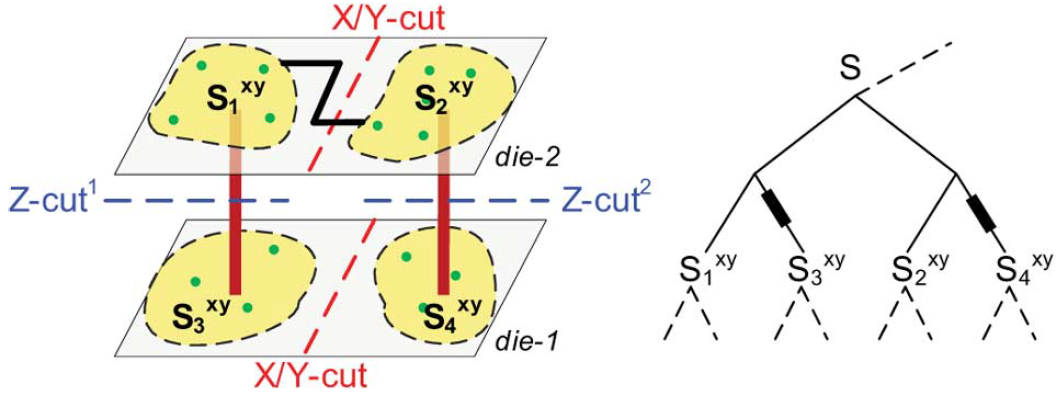
\includegraphics[width=1\linewidth]{img/cuts.png}
	\centering
	\caption{X/Y-cut followed by two Z-cuts. Source: \cite{b2}}
	\label{fig:cuts}
\end{figure}

The algorithm is finished when each sink is in its own set. The result of the algorithm for a two die IC under various TSV bounds is shown in Fig. \ref{fig:tree_examples}.

\begin{figure}[htbp]
	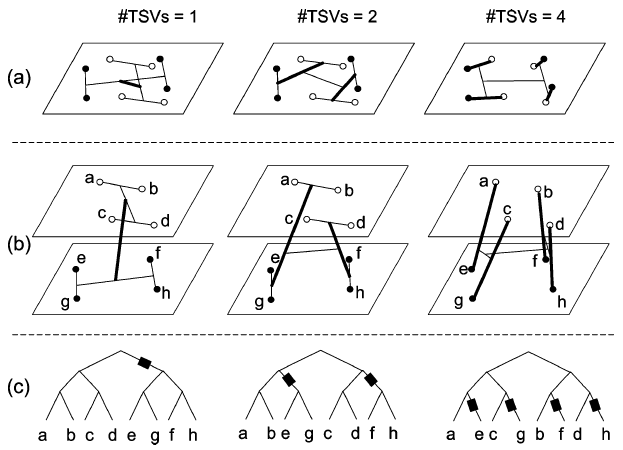
\includegraphics[width=1\linewidth]{img/tree_examples.png}
	\centering
	\caption{The 3D abstract tree generation under various TSV bounds. (a) shows a top view, (b) shows a 3D view and (c) show the resulting binary tree where the squares denote TSVs. Source: \cite{b2}}
	\label{fig:tree_examples}
\end{figure}

After the binary tree is calculated, the slew-aware buffering and embedding takes place.

\subsection{Impact of the TSV count on the clock power}
The more TSVs are used, the smaller becomes the overall wire length. This leads to a smaller wire RC and therefore the ciruit consumes less power. But after a certain point the capacitance of the inserted TSVs are too large what then results in an increasing power consumtion. Hence, there is a minimum power point for a certain number of TSVs. This point can be found by sweeping the TSV bound in the simulation as it was done for Fig. \ref{fig:tsv_sweep}.

\begin{figure}[htbp]
	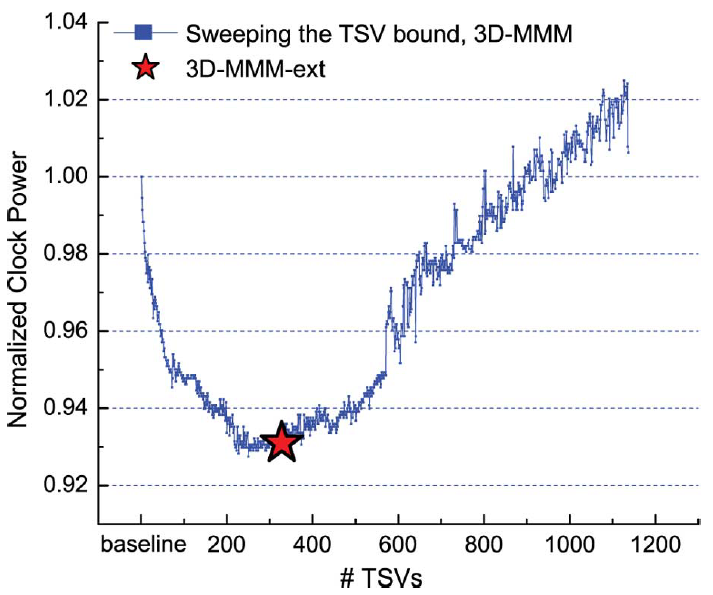
\includegraphics[width=1\linewidth]{img/tsv_sweep.png}
	\centering
	\caption{Clock power over TSV count for a two die stack using 100fF TSVs. The red star denotes the predictet optimum power point found by 3D-MMM-ext algorith which was developed in \cite{b2}. Source: \cite{b2}}
	\label{fig:tsv_sweep}
\end{figure}

The exhaustive search by sweeping the TSV bound is often not practicable due to its time-consuming runtime. For this reason X. Zhao et al. \cite{b2} developed the 3D-MMM-ext algorithm that can predict the minimum power point in a good manner. Morover, X. Zhao et al. showed that using the optimal TSV count can save up to 36\% of the total power consumed by six-die stacked IC.


\section{Conclusion}
As a conclusion one can say that a well designed clock network can save a lot of power. This can be achieved by voltage scaling, but in this case the clock network has to be designed in different way than it would be done for a super-threshold regime. M. Seok et al. showed that for ULV applications unbuffered clock trees consume less power and are in addition to that more robust to MOSFET process variations and therfore show a better skew and slew behaviour.

For nowadays 3D staced ICs, there is an optimal number of TSVs regarding the power consumtion. This is because more TSVs can reduce the overall wire lenght (and therefore the wire RC), but too many TSVs lead to a too large capacitance.

So we can finally conclude that the consumed power by the clock can drastically be reduced by choosing the optimal routing topology. Afterwards, the power can still be reduced by measures such as voltage scaling.

%\subsection{Figures and Tables}
%\paragraph{Positioning Figures and Tables} Place figures and tables at the top and 
%bottom of columns. Avoid placing them in the middle of columns. Large 
%figures and tables may span across both columns. Figure captions should be 
%below the figures; table heads should appear above the tables. Insert 
%figures and tables after they are cited in the text. Use the abbreviation 
%``Fig.~\ref{fig}'', even at the beginning of a sentence.

%\begin{table}[htbp]
%\caption{Table Type Styles}
%\begin{center}
%\begin{tabular}{|c|c|c|c|}
%\hline
%\textbf{Table}&\multicolumn{3}{|c|}{\textbf{Table Column Head}} \\
%\cline{2-4} 
%\textbf{Head} & \textbf{\textit{Table column subhead}}& \textbf{\textit{Subhead}}& \textbf{\textit{Subhead}} \\
%\hline
%copy& More table copy$^{\mathrm{a}}$& &  \\
%\hline
%\multicolumn{4}{l}{$^{\mathrm{a}}$Sample of a Table footnote.}
%\end{tabular}
%\label{tab1}
%\end{center}
%\end{table}

%\begin{figure}[htbp]
%\centerline{\includegraphics{fig1.png}}
%\caption{Example of a figure caption.}
%\label{fig}
%\end{figure}

\begin{thebibliography}{00}
\bibitem{b1} J.Zhou, T.H.Kim and Y.Lian, ``Near-threshold processor design techniques for power-constrained 
computing devices,'' 2017 IEEE 12th International Conference on ASIC (ASICON), Guiyang, China, 2017, pp.920-923
\bibitem{b2} J. Tang, C. Liu, Y. L. Chou and S. Liu, ``OCP: Offload Co-Processor
for energy efficiency in embedded mobile systems,'' 2013 IEEE 24th International Conference on Application-Specific 
Systems, Architectures and Processors, Washington, DC, 2013, pp. 107-110
\bibitem{b3}
\bibitem{b4}
\bibitem{b5}
\bibitem{b6}
\bibitem{b7}
\end{thebibliography}
\end{document}
